% S&A Latex Template for Assignment Docs
% Reinhold Preiner, 2024
%-------------------------------------------------------------------

\documentclass{article}
\usepackage[utf8]{inputenc}
\usepackage{hyperref}
\usepackage{cite}
\usepackage[english]{babel}
\usepackage{hyperref}
\usepackage{subfig}
\usepackage{graphicx}
\usepackage{float}

\usepackage{geometry}
\geometry{margin=1in}

\hypersetup{
    colorlinks=true,
    linkcolor=blue,
    filecolor=magenta,      
    urlcolor=cyan,
    citecolor = black,
}

\setlength{\parindent}{0pt}
\setlength{\parskip}{0.5em}

\usepackage{comment}

\title{	
	\large Simulation \& Animation - SS 2025\\
	\Huge{Binding of glass Mini golf 2}\\
	\huge{Can you hit it?}
}
\author{\parbox{\textwidth}{\centering
	Florian Winston, 11727495, winston@student.tugraz.at\\%
	Leon Tiefenboeck, 11919874, tiefenboeck@student.tugraz.at\\%
}}
\date{\today}


\begin{document}

\maketitle

\begin{figure}[H]
    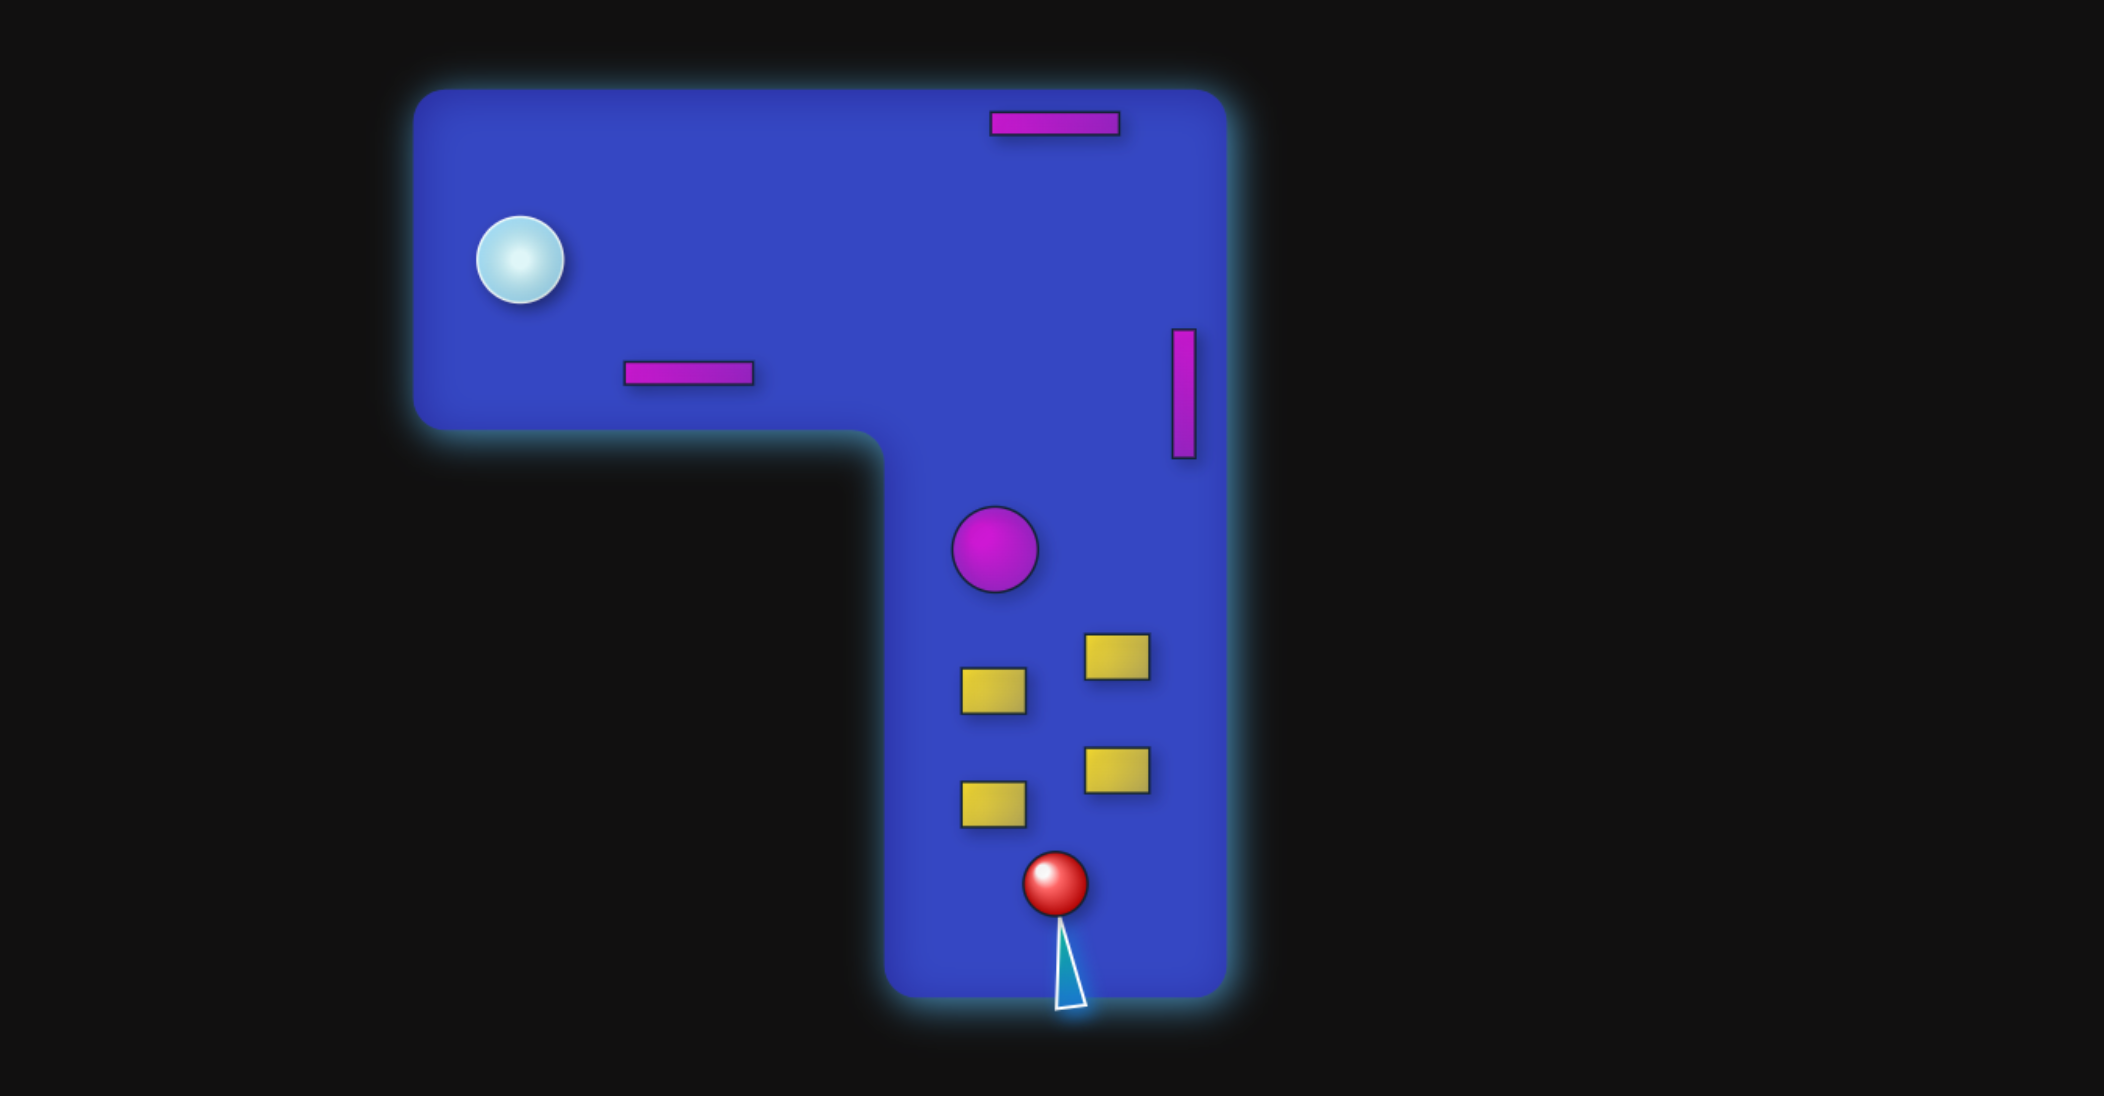
\includegraphics[width=\textwidth]{showcase.png}
    \caption{Screenshot of the level 1}
\end{figure}

\section{User Documentation}

\subsection{Gameplay Overview}

In our game are three possible levels to be played which feature different techniques: the first contains rigid body collision and path interpolation, the second particle dynamics and the third voronoi fracture. 
The main concept is the same in all levels, namely putting the small red ball into the white glowing hole. 
In each level this is achieved by using the respective technique.

\subsection{Controls}

The game is started by opening \texttt{main.html} which opens a 
start screen where one can choose between the three levels. 

When starting a level you see, at the bottom of the screen, the ball. This ball can be moved 
by clicking it, dragging somewhere and then releasing the mouse button. 
The ball will move in the opposite direction of where was dragged and the momentum of the 
ball depends on how far back was dragged, much like a spring. This is indicated by an arrow that appears below the ball.
Somewhere else in the game area there is a hole, which, to set it apart from the other game objects, 
is very bright and glows a little bit. This is the hole 
the ball should go into. If the player manages that, the level is completed.
On the left side of the screen there is the control panel where level specific techs 
and the overall animation rate and render rate can be adjusted. Here one can also toggle the visualizations 
for different techs. 
Lastly the game can be paused by pressing the \texttt{Escape} key and resumed by pressing it again.

\section{Technical Documentation}

\subsection{General Structure}
We implemented our game in a very modular way. We have two main game classes that control the game logic 
and everything that is the same in each level. There are two, since we realized that using different classes would be simpler than making one class work for all techs. These classes also includes one main loop that 
updates the position of objects and renders them. We can very easily add other objects from other parts in the 
code to this loop. We can adjust the animation update rate here 
by simply adding a delay to when the next iteration of this loop is called. 
We achieve the frame rate independence also here, by calculating how long a frame took to produce 
and then adjust all updates by this delta. 

Next we have an individual class for each of the techs. Here everything should 
also be confined and other parts of the game need only interact with the constructor
and the \texttt{update} and \texttt{render} methods.

Finally, we have a file for each level that interacts with the main game 
class and the different techs. Here we set up
the game objects that are controlled by a tech and their controls (visualization, speed adjustment, etc.).

\subsection{Path Interpolation}

This is shown in level 1. Some of the objects (colored in pink) are moving along a spline path. 
To construct a spline we basically only need the control points, that an object should go through, and an 
object that moves along this spline. Here theoretically we could always just draw a simple circle but 
for our game we wanted that the main ball can bounce off the path interpolated objects, so we used stationary rigid bodies
as the moving objects. More on this later, but these are basically rigid bodies that can only 
exert forces on other objects but do not move themselves, i.e. their entire movement is controlled by the spline.

For our splines we also have the option to change the traversal speed, to loop them or move them back and forth and 
to use easing function to move the objects at non-constant speeds.

Then we set the t values (basically how far along the spline we are) to $0$ and 
precompute the arc length table. Then the spline is ready and waits until \texttt{update} is called. 
In \texttt{update} we calculate the new value based on the current t value and the speed and then we make the 
lookup in the arc length table and evaluate the spline at that value. We also have a render function 
that just draws a circle at the current position (though in the future we also want to add different shapes).

\subsection{Rigid-Body Dynamics}

\subsection{Particle Dynamics}
Level 2 showcases particle dynamics. Here there are two repelling bodies in red and two attracting bodies in purple. Once the ball is shot, they start affecting it. The force field created by the bodies and trajectory of the ball over the last few seconds can be visualized through the button. One can also change the integration method to choose between the RK4 and Euler methods. Only the ball is effected by the forces, while there is no effect on the other object from each other or from the ball.  \newline

The code for this is located in the ParticleDynamics.js file. There, the particle class with the necessary members is defined. It also holds the defineForces function, which takes all the particles into account, to calculate the effect they have onto the ball. The Rk4 an euler functions are used for the integration step and apply the results to the ball. The visualize and drawArrow functions are used to draw the particles, the trail and the force field. 
Note: Pushing the visualization button once visualizes the trail, pushing again adds the field. Pushing a third time only visualizes the field and pushing a fourth time turns the visualization off again. 
A vector class is also defined, which will be integrated into the other techs. 

\subsection{Voronoi Fracture}
Level 3 showcases the Vornonoi Fracture. The fractured object is an octagon. When the ball gets close to it, the process of fracture starts. The visualization button can be used after the object fractures. It first shows the seed points, then the intersection of the distance field between the mesh and the Voronoi distance field. When hit again, first the seed points and then the field are deactivated. The visualization is only available after the collision, since the slides specified, that the fragmentation calculations should be performed at runtime after impact. The toggle noise button can be pressed before the collision to enable or disable the fracture with noise in the Voronoi fields.

The code for this is located in VoronoiFracture,js. There the "Voronoi" class is defined which holds all the necessary data and methods. On start the image for the object is loaded. Once the ball is close enough to the object, the Voronoi seeds are distributed randomly in a bounding box around the object and Perlin noise with the same bounding box is calculated. Next, the SDF is calculated by iterating over all pixels in the bounding box. Here the noise is added to the location of the pixels. After that the mesh of the object is defined and its SDF calculated. Next, the intersection of both SDFs is created and used to calculate which pixels belong to which fragment. Each pixel gets its color values from the image. Finally, the fragments are assigned random velocities, which are scaled by the animation rate. Through this, after impact the object fragments with each part moving seemingly randomly

\end{document}